%%%%%%%%%%%%%%%%%%%%%%%%%%%%%%%%%%%%%%%%%%%%%%%%%%%%%%%%%%%%%%%%%%%%%%%%%%%%%%%%
%%%%%%%%%%%%%%%%%%   Vorlage für eine Abschlussarbeit   %%%%%%%%%%%%%%%%%%%%%%%%
%%%%%%%%%%%%%%%%%%%%%%%%%%%%%%%%%%%%%%%%%%%%%%%%%%%%%%%%%%%%%%%%%%%%%%%%%%%%%%%%

% Erstellt von Maximilian Nöthe, <maximilian.noethe@tu-dortmund.de>
% ausgelegt für lualatex und Biblatex mit biber

% Kompilieren mit
% lualatex dateiname.tex
% biber dateiname.bcf
% lualatex dateiname.tex
% lualatex dateiname.tex
% oder einfach mit:
% make

\documentclass[
  tucolor,
  BCOR=12mm,     % 12mm binding corrections, adjust to fit your binding
  parskip=half,  % new paragraphs start with half line vertical space
  open=any,      % chapters start on both odd and even pages
  cleardoublepage=plain,  % no header/footer on blank pages
]{tudothesis}


% Warning, if another latex run is needed
\usepackage[aux]{rerunfilecheck}

% just list chapters and sections in the toc, not subsections or smaller
\setcounter{tocdepth}{1}

%------------------------------------------------------------------------------
%------------------------------ Sprache und Schrift: --------------------------
%------------------------------------------------------------------------------
\usepackage{fontspec}
\defaultfontfeatures{Ligatures=TeX}  % -- becomes en-dash etc.

% german language
\usepackage{polyglossia}
\setdefaultlanguage{english}

% for english abstract and english titles in the toc
\setotherlanguages{german}

% intelligent quotation marks, language and nesting sensitive
\usepackage[autostyle]{csquotes}

% microtypographical features, makes the text look nicer on the small scale
\usepackage{microtype}

%------------------------------------------------------------------------------
%------------------------ Für die Matheumgebung--------------------------------
%------------------------------------------------------------------------------

\usepackage{amsmath}
\usepackage{amssymb}
\usepackage{mathtools}

% Enable Unicode-Math and follow the ISO-Standards for typesetting math
\usepackage[
  math-style=ISO,
  bold-style=ISO,
  sans-style=italic,
  nabla=upright,
  partial=upright,
]{unicode-math}
\setmathfont{Latin Modern Math}

% nice, small fracs for the text with \sfrac{}{}
\usepackage{xfrac}


%------------------------------------------------------------------------------
%---------------------------- Numbers and Units -------------------------------
%------------------------------------------------------------------------------

\usepackage[
  locale=UK,
  separate-uncertainty=true,
  per-mode=symbol-or-fraction,
]{siunitx}
\sisetup{math-micro=\text{µ},text-micro=µ}

%------------------------------------------------------------------------------
%-------------------------------- tables  -------------------------------------
%------------------------------------------------------------------------------

\usepackage{booktabs}       % stellt \toprule, \midrule, \bottomrule

%------------------------------------------------------------------------------
%-------------------------------- graphics -------------------------------------
%------------------------------------------------------------------------------

\usepackage{graphicx}
\usepackage{grffile}

% allow figures to be placed in the running text by default:
\usepackage{scrhack}
\usepackage{float}
\floatplacement{figure}{htbp}
\floatplacement{table}{htbp}

% keep figures and tables in the section
\usepackage[section, below]{placeins}


%------------------------------------------------------------------------------
%---------------------- customize list environments ---------------------------
%------------------------------------------------------------------------------

\usepackage{enumitem}

%------------------------------------------------------------------------------
%------------------------------ Bibliographie ---------------------------------
%------------------------------------------------------------------------------

\usepackage[
  backend=biber,   % use modern biber backend
  autolang=hyphen, % load hyphenation rules for if language of bibentry is not
                   % german, has to be loaded with \setotherlanguages
                   % in the references.bib use langid={en} for english sources
]{biblatex}
\addbibresource{references.bib}  % die Bibliographie einbinden
\DefineBibliographyStrings{english}{andothers = {{et\,al\adddot}}}

%------------------------------------------------------------------------------
%------------------------------ Sonstiges: ------------------------------------
%------------------------------------------------------------------------------

\usepackage[pdfusetitle,unicode,linkbordercolor=tugreen]{hyperref}
\usepackage{bookmark}
\usepackage[shortcuts]{extdash}

%------------------------------------------------------------------------------
%-------------------------    Angaben zur Arbeit   ----------------------------
%------------------------------------------------------------------------------

\author{Jan Moritz Behnken}
\title{Gamma-Hadron Separation with Deep Learning for the First G-APD Cherenkov Telescope}
\date{2017}
\birthplace{Achim}
\chair{Lehrstuhl für Experimentelle Physik V}
\division{Fakultät Physik}
\thesisclass{Bachelor of Science}
\submissiondate{15. September 2017}
\firstcorrector{Prof.~Dr.~Dr.~Wolfgang~Rhode}
\secondcorrector{Prof.~Dr.~Kevin~Kröninger}

% tu logo on top of the titlepage
\titlehead{
\includegraphics[height=1.5cm]{logos/tu-logo.pdf}}

\begin{document}
\frontmatter
% \thispagestyle{empty}
\setcounter{page}{2}
\section*{Hinweise}
Empfohlen wird die Verwendung dieser Vorlage mit der jeweils aktuellsten TeXLive Version (Linux, Windows) bzw. MacTeX Version (MacOS).
Aktuell ist dies TeXLive 2016. Download hier:
\begin{center}
  \ttfamily\url{https://www.tug.org/texlive/}
\end{center}
Bei Verwendung von TexLive Versionen 2014 und älter sollte
die Zeile
\begin{center}
\verb+\RequirePackage{fixltx2e}+ 
\end{center}
als erste Zeile der Präambel noch vor der Dokumentenklasse eingefügt werden.
Dies lädt diverse Bugfixes für LaTeX, die ab TexLive 2015 Standard sind.

Die Vorlage \texttt{thesis.tex} ist für die Kompilierung mit \texttt{lualatex} ausgelegt, mit wenigen Anpassungen kann sie aber auch mit \texttt{pdflatex} oder \texttt{xelatex} verwendet werden. 
Die Dokumentenklasse \texttt{tudothesis.cls} kann mit allen drei Programmen verwednet werden.

Achten Sie auch auf die Kodierung der Quelldateien.
Bei Verwendung von Xe\LaTeX\ oder Lua\LaTeX\ (empfohlen) müssen die
Quelldateien UTF-8 kodiert sein.
Bei Verwendung von pdf\LaTeX\ nutzen Sie die Pakete \texttt{inputenc} und \texttt{fontenc} mit der korrekten Wahl der Kodierungen.

Eine aktuelle Version dieser Vorlage steht unter 
\begin{center}
  \ttfamily\url{https://github.com/maxnoe/tudothesis}
\end{center}
zur Verfügung.

Alle verwendeten Pakete werden im \LaTeX{} Kurs von Pep et al.\ erklärt:
\begin{center}
  \ttfamily\url{http://toolbox.pep-dortmund.org/notes}
\end{center}

Für Rückmeldungen und bei Problemen mit der Klasse oder Vorlage, bitte ein \emph{Issue} auf GitHub aufmachen oder eine Email an
\href{mailto:maximilian.noethe@tu-dortmund.de}{maximilian.noethe@tu-dortmund.de} schreiben.

Wenn Sie die Dokumentenklasse mit der Option \texttt{tucolor} laden, werden verschiedene Elemente in TU-Grün gesetzt.

\maketitle

% Gutachterseite
\makecorrectorpage

% hier beginnt der Vorspann, nummeriert in römischen Zahlen
\thispagestyle{plain}

\section*{Abstract}
High energetic particles from cosmic sources reach the aerosphere and interact with it.
Thereby caused particle showers emit Cherenkov radiation, which can be recorded by telescopes at ground-level.

This thesis is motivated by the study of these images from the FACT telescope through Deep Learning.
To identify the source of the particles a separation of images caused by gamma rays and hadrons will be realised.
Therefor a simulated dataset is used to train a Convolutional Neural Network (CNN).
To come close to the ideal performance \num{30} different network architectures and regularizations are being compared to each other.

Afterwards a comparison is drawn between the performance of the currently used classifier and the CNN.
Although the CNN performs comparable on a test dataset, it clearly fails to separate gamma rays from hadrons at real measured images.
This can be reduced to a systematic error between simulated and real datasets (Monte Carlo Mismatch).

\section*{Kurzfassung}
\begin{german}
Von kosmischen Quellen erreichen energiereiche Teilchen die obersten Schichten der Erdatmosphäre und wechselwirken mit dieser.
Dabei entstehende Teilchenschauer senden Tscherenkov-Strahlung aus, welche von Teleskopen am Erdboden aufgenommen werden kann.

Motivation für diese Arbeit ist die Untersuchung dieser Bilder vom FACT-Teleskop mittels Deep Learning.
Um die Quellen der Teilchen ausfindig zu machen, werden die durch Gammastrahlung und Hadronen ausgelösten Bilder separiert.
Hierfür wird auf simulierten Datensätzen ein Convolutional Neural Network (CNN) trainiert.
Um der optimalen Performance nahe zu kommen werden \num{30} unterschiedliche Netzwerkarchitekturen und Regularisierungen miteinander verglichen.

Anschließend wird ein Vergleich der Performance zwischen dem bisher eingesetzten Klassifizierer und dem CNN gezogen.
Obwohl das CNN auf Testddaten eine vergleichbar gute Leistung erreicht,
zeigt sich ein deutliches Versagen beim Separieren von real gemessenen Bildern.
Dies wird auf einen systematischen Fehler zwischen simulierten und echten Daten zurückgeführt (Monte Carlo Mismatch).
\end{german}

\tableofcontents

\mainmatter
% Hier beginnt der Inhalt mit Seite 1 in arabischen Ziffern
\chapter{Introduction}
The topic of this thesis belongs to an astrophysical subsection investigating some of the most extreme phenomena in the Universe.
For example black holes, supernovae and pulsars are known to be sources of high energetic particles,
but the events emitting this radiation are still a subject of research.
To deepen the knowledge concerning these events the emitted gamma rays and hadrons can be examined by telescopes.

The advantage of gamma rays over likewise emitted hadrons is their indivertible nature against electromagnetic fields.
Whereas the direction of hadrons is scrambled by magnetic fields while passing galaxies and nebulas, gamma rays are immune.
When the sub-atomic particles arrive at the earth the direction of the gamma rays is still preserved
and can be used to detect and measure their source.

When entering the aerosphere gamma rays as well as hadrons collide with other particles
and transfer some of their energy to their collision partners.
Both particles cause air showers which emit Tcherenkov radiation by reason of the high energies involved.
Ground-level telesopes can measure the gamma rays and hadrons indirectly by observing the brief Tcherenkov flash.

Afterwards machine learning algorithms classify the recorded images as being triggered by a gamma ray or a hadron.
Using only the measurements caused by gamma rays their preserved direction displays their cosmic source.
Further investigation of these gamma events can reveal source specific characteristics.

This thesis will take a look into Deep Learning and Convolutional Neural Networks to find a better classification algorithm.
Different network architectures will be evaluated and their hyperparameters will be optimized.
Finally the best model will be compared to the currently used classifier.

\chapter{Theoretical foundations}


\section{Cosmic radiation}
The cosmos is filled with particles of many kinds and sources.
Whereas the travel direction of charged particles is constantly bend by electromagnetic fields on their journey through space,
uncharged particles like gamma rays preserve their direction during their voyage.
This circumstances allow to identify their source.
Source specific characteristics can be found by determining the particle's properties.

\begin{figure}
    \centering
    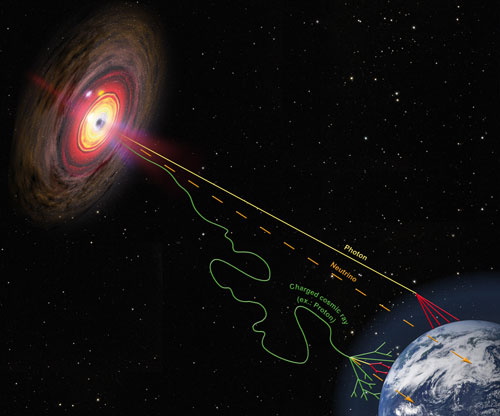
\includegraphics[width=9cm]{Plots/cosmic_ray.jpg}
    \caption{Charged and uncharged particles propagation through space}
    \label{fig:cosmic_ray}
\end{figure}

Gamma particles as well as hadrons can not cut through the earth's aerosphere and collide therefore with it.
Upon this collision the cosmic particle transfers some of its energy the its collision partner.
This causes an air shower by reason of the high energies of 0-0eV? involved.
Since the speed of light in air is lower than in space some air shower particles can be faster than the light speed in air
without violating the cosmic speed of light.
In this case those particles emit a cone of Tcherenkov radiation caused by the identically named effect.
When a high energetic cosmic particle interacts with the aerosphere, a short flash of Tcherenkov light can be detected at ground-level.

\begin{figure}
    \centering
    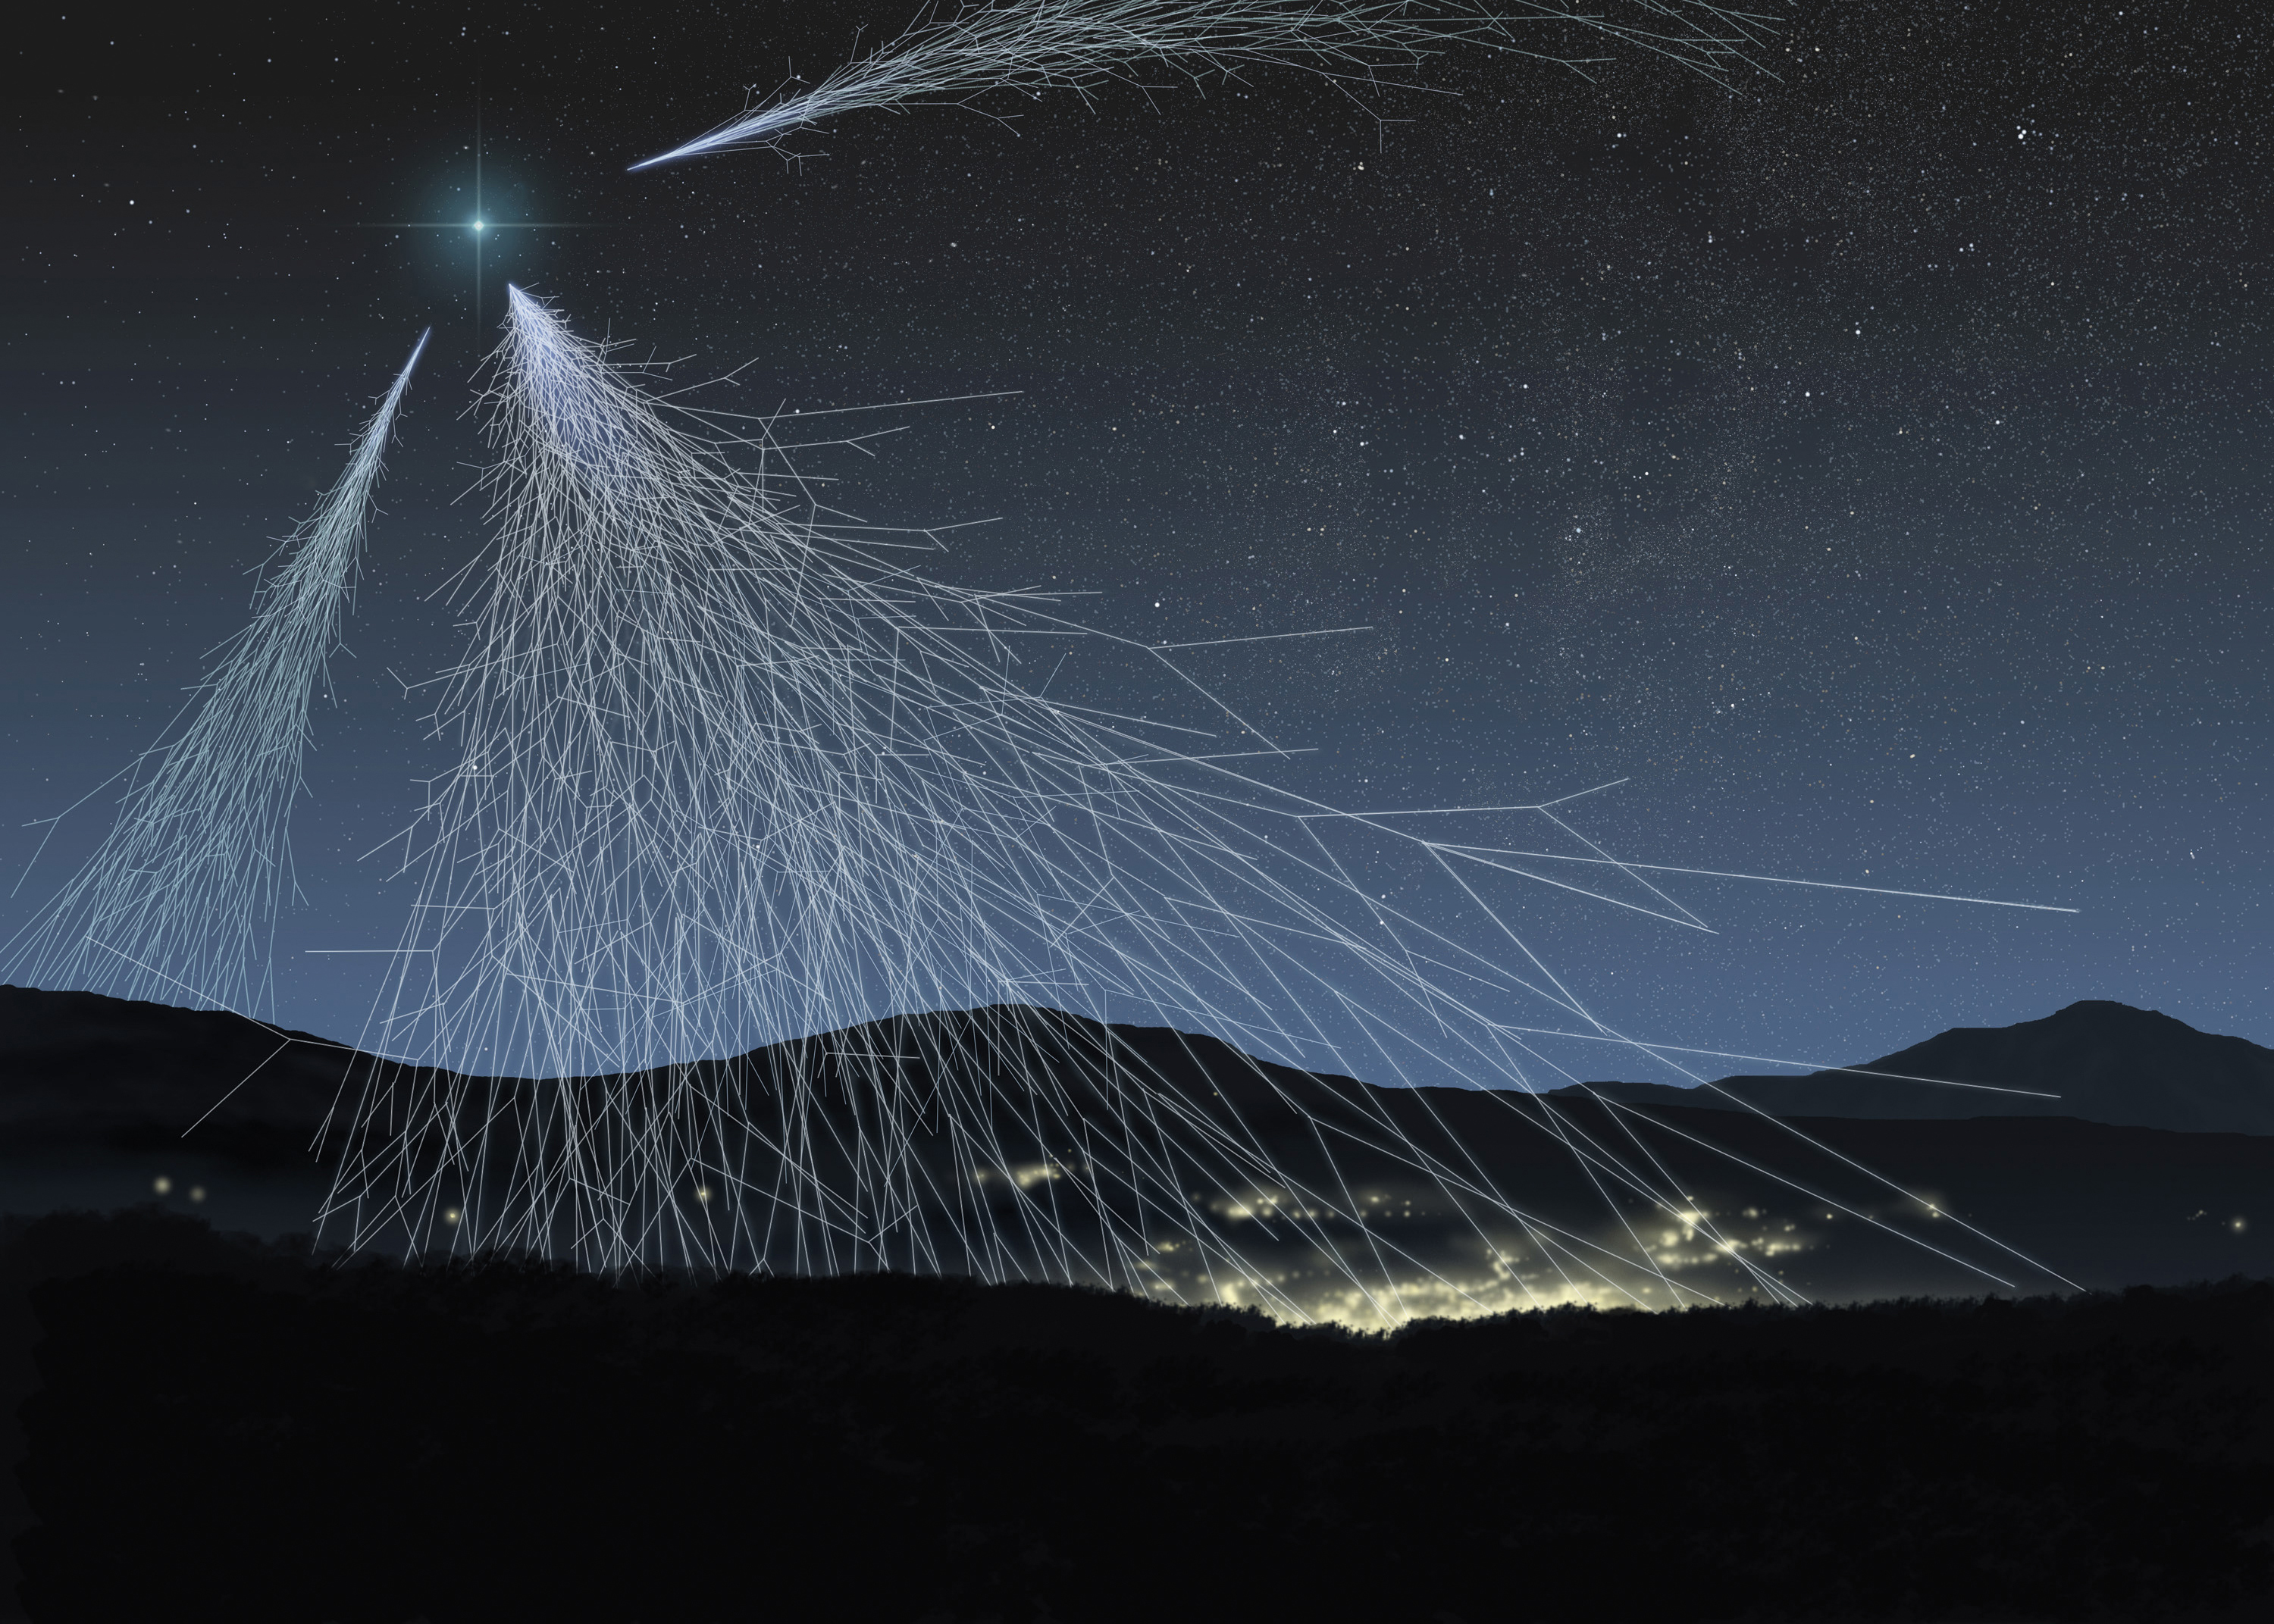
\includegraphics[width=9cm]{Plots/air_shower.jpg}
    \caption{Gamma ray causing an air shower in the aerosphere which emits Tcherenkov light}
    \label{fig:air_shower}
\end{figure}


\section{FACT telescope}
Among other telescopes the First G-APD Cherenkov Telescope (FACT) on La Palma records these light flashes.
It uses Geiger-mode avalanche photodiods (G-APDs) as photo sensors for a test benchmark of this technology.
With its small mirror surface of 9.5 sqm it operates since 2011
and collects data of air showers caused by cosmic radiation in the TeV energy range.

The 1440 camera pixel form a hexagonal grid.
This hexagonal pixel structure represents a challenge for the further image processing
since software for image classification was developed for images with quadratic pixels.
Therefor the camera image has to be transformed by using the pixel ids to map the hexagonal to a quadratic grid structure.
Skewing the image and padding it with empty pixels enables further processing without developing special software.
One drawback of this procedure is the loss of some direct neighborhood information
(hexagonal: 6 neighbors, quadratic: 4 neighbors) of every pixel.

\begin{figure}
    \centering
    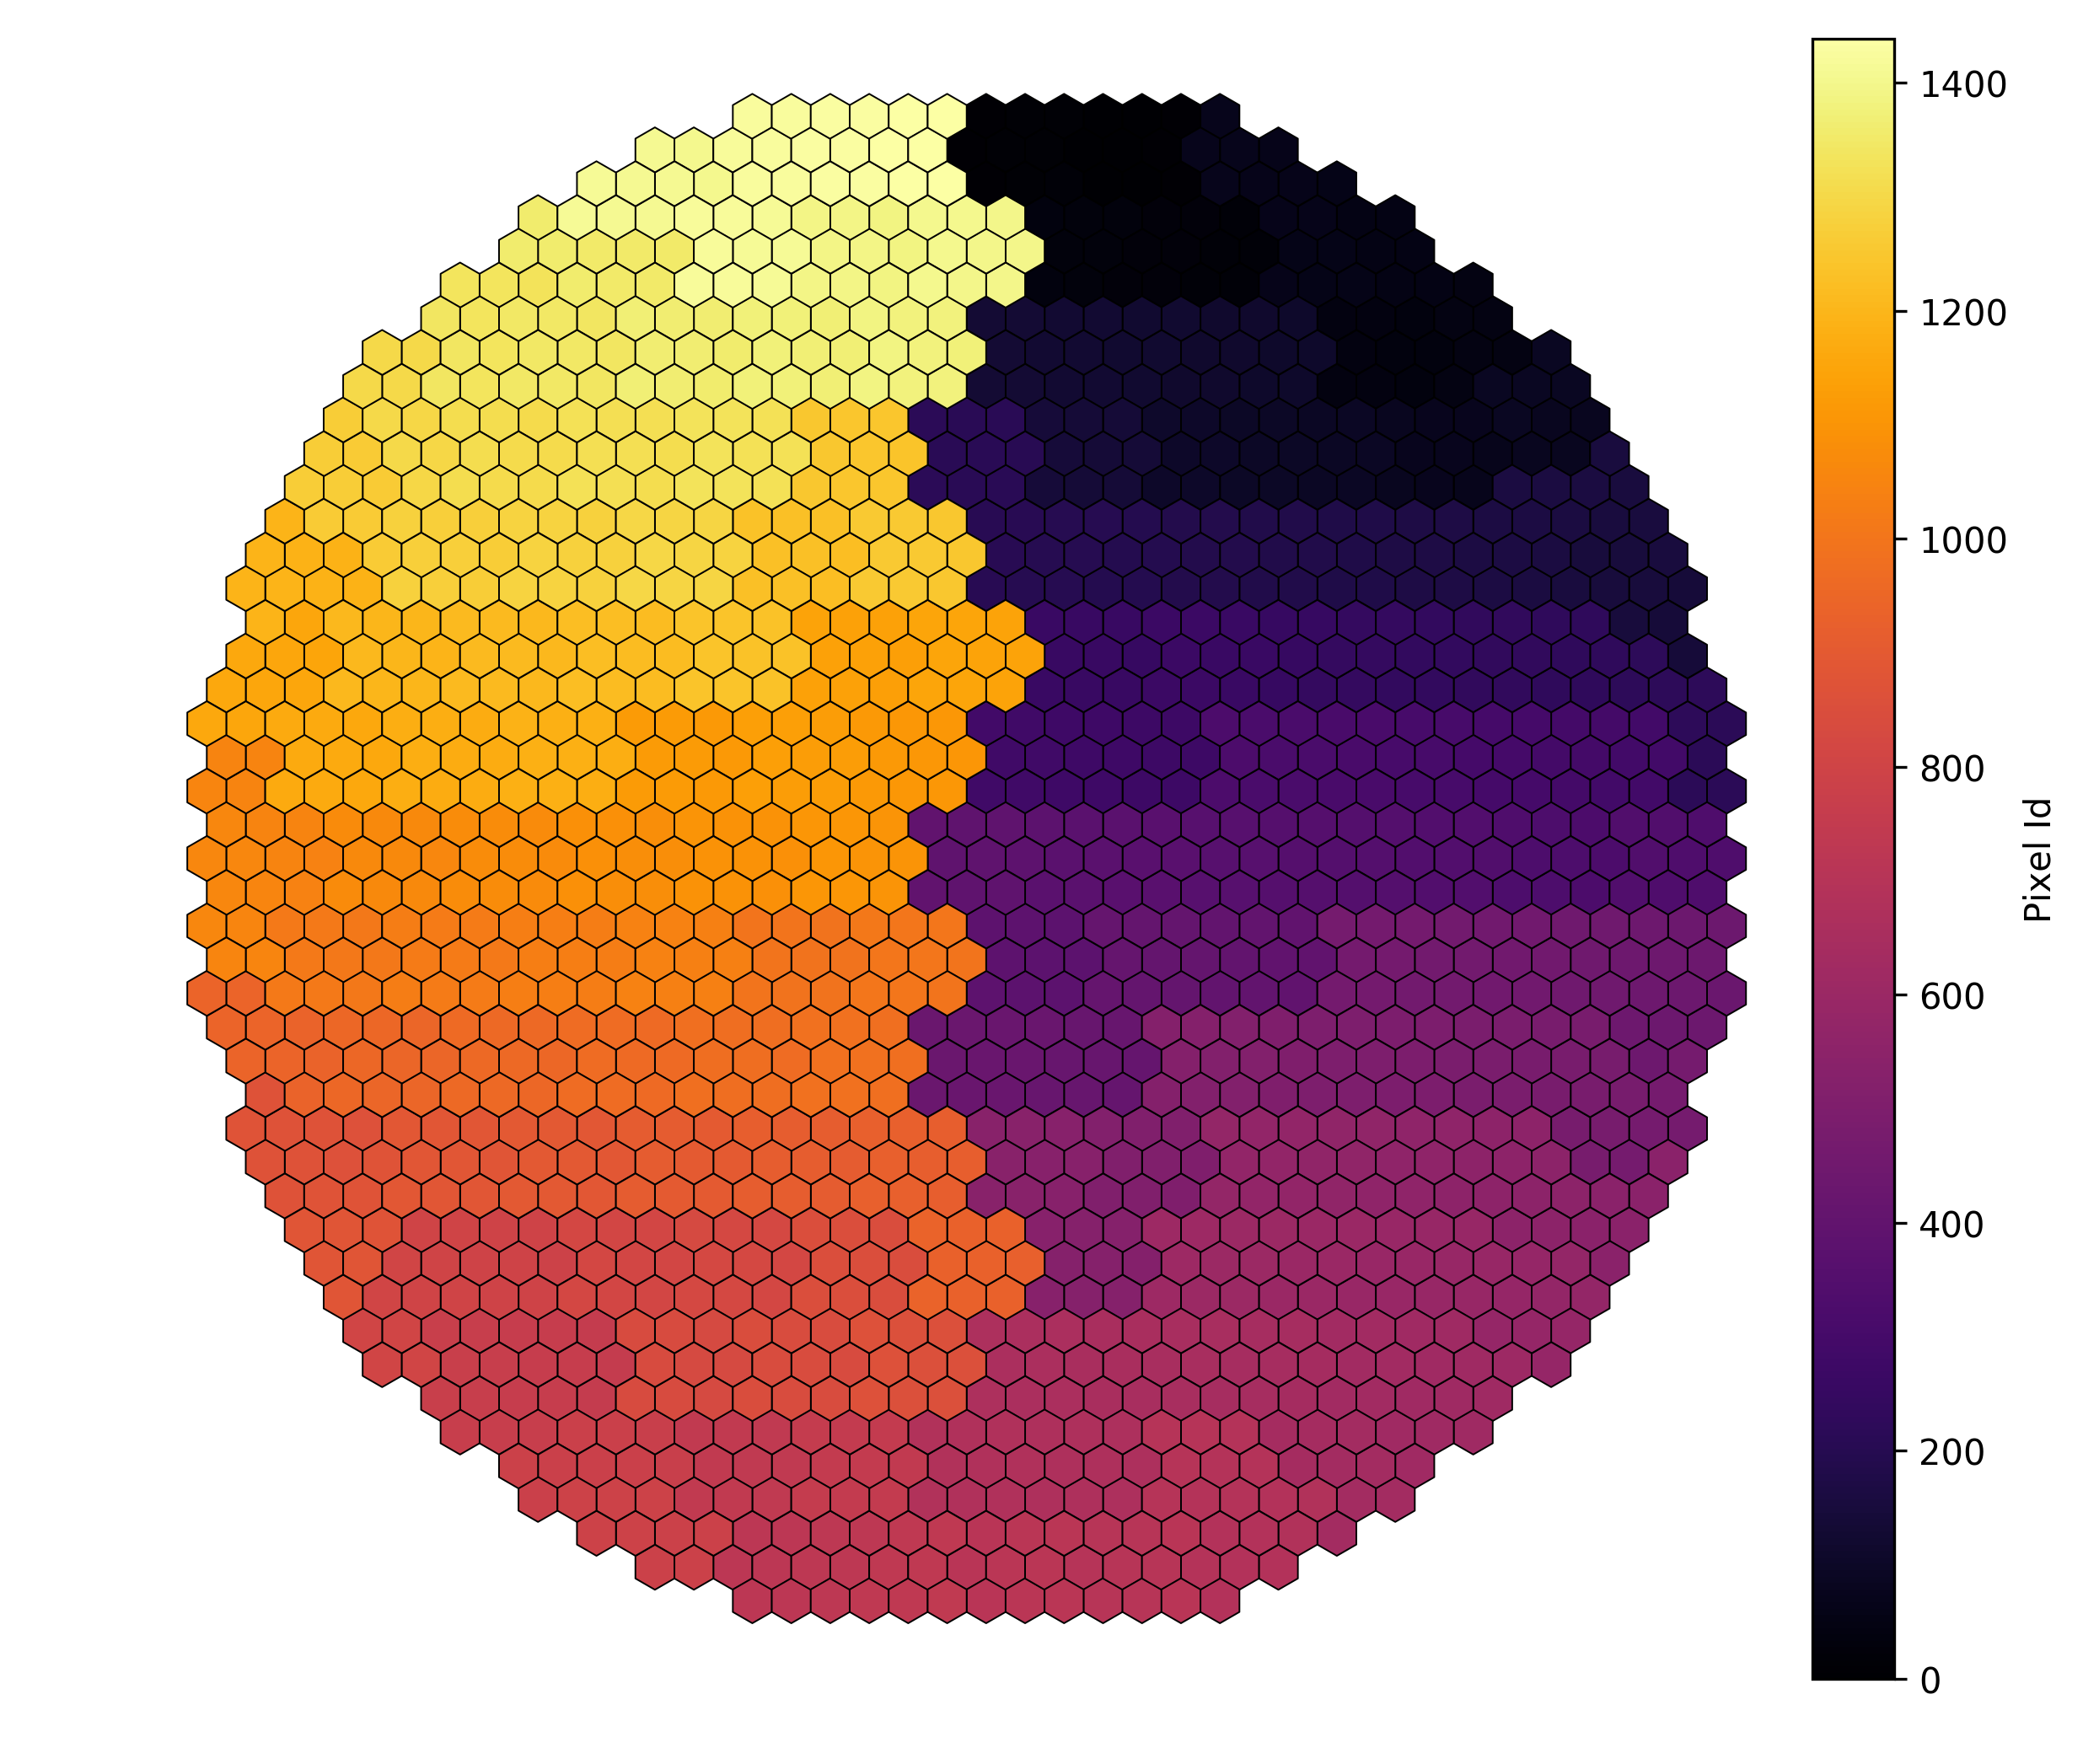
\includegraphics[width=6cm]{Plots/FACT_Image.png}
    \caption{FACT camera image with hexagonal pixels and the mapping axes}
    \label{fig:fact_image}
\end{figure}

\begin{figure}
    \centering
    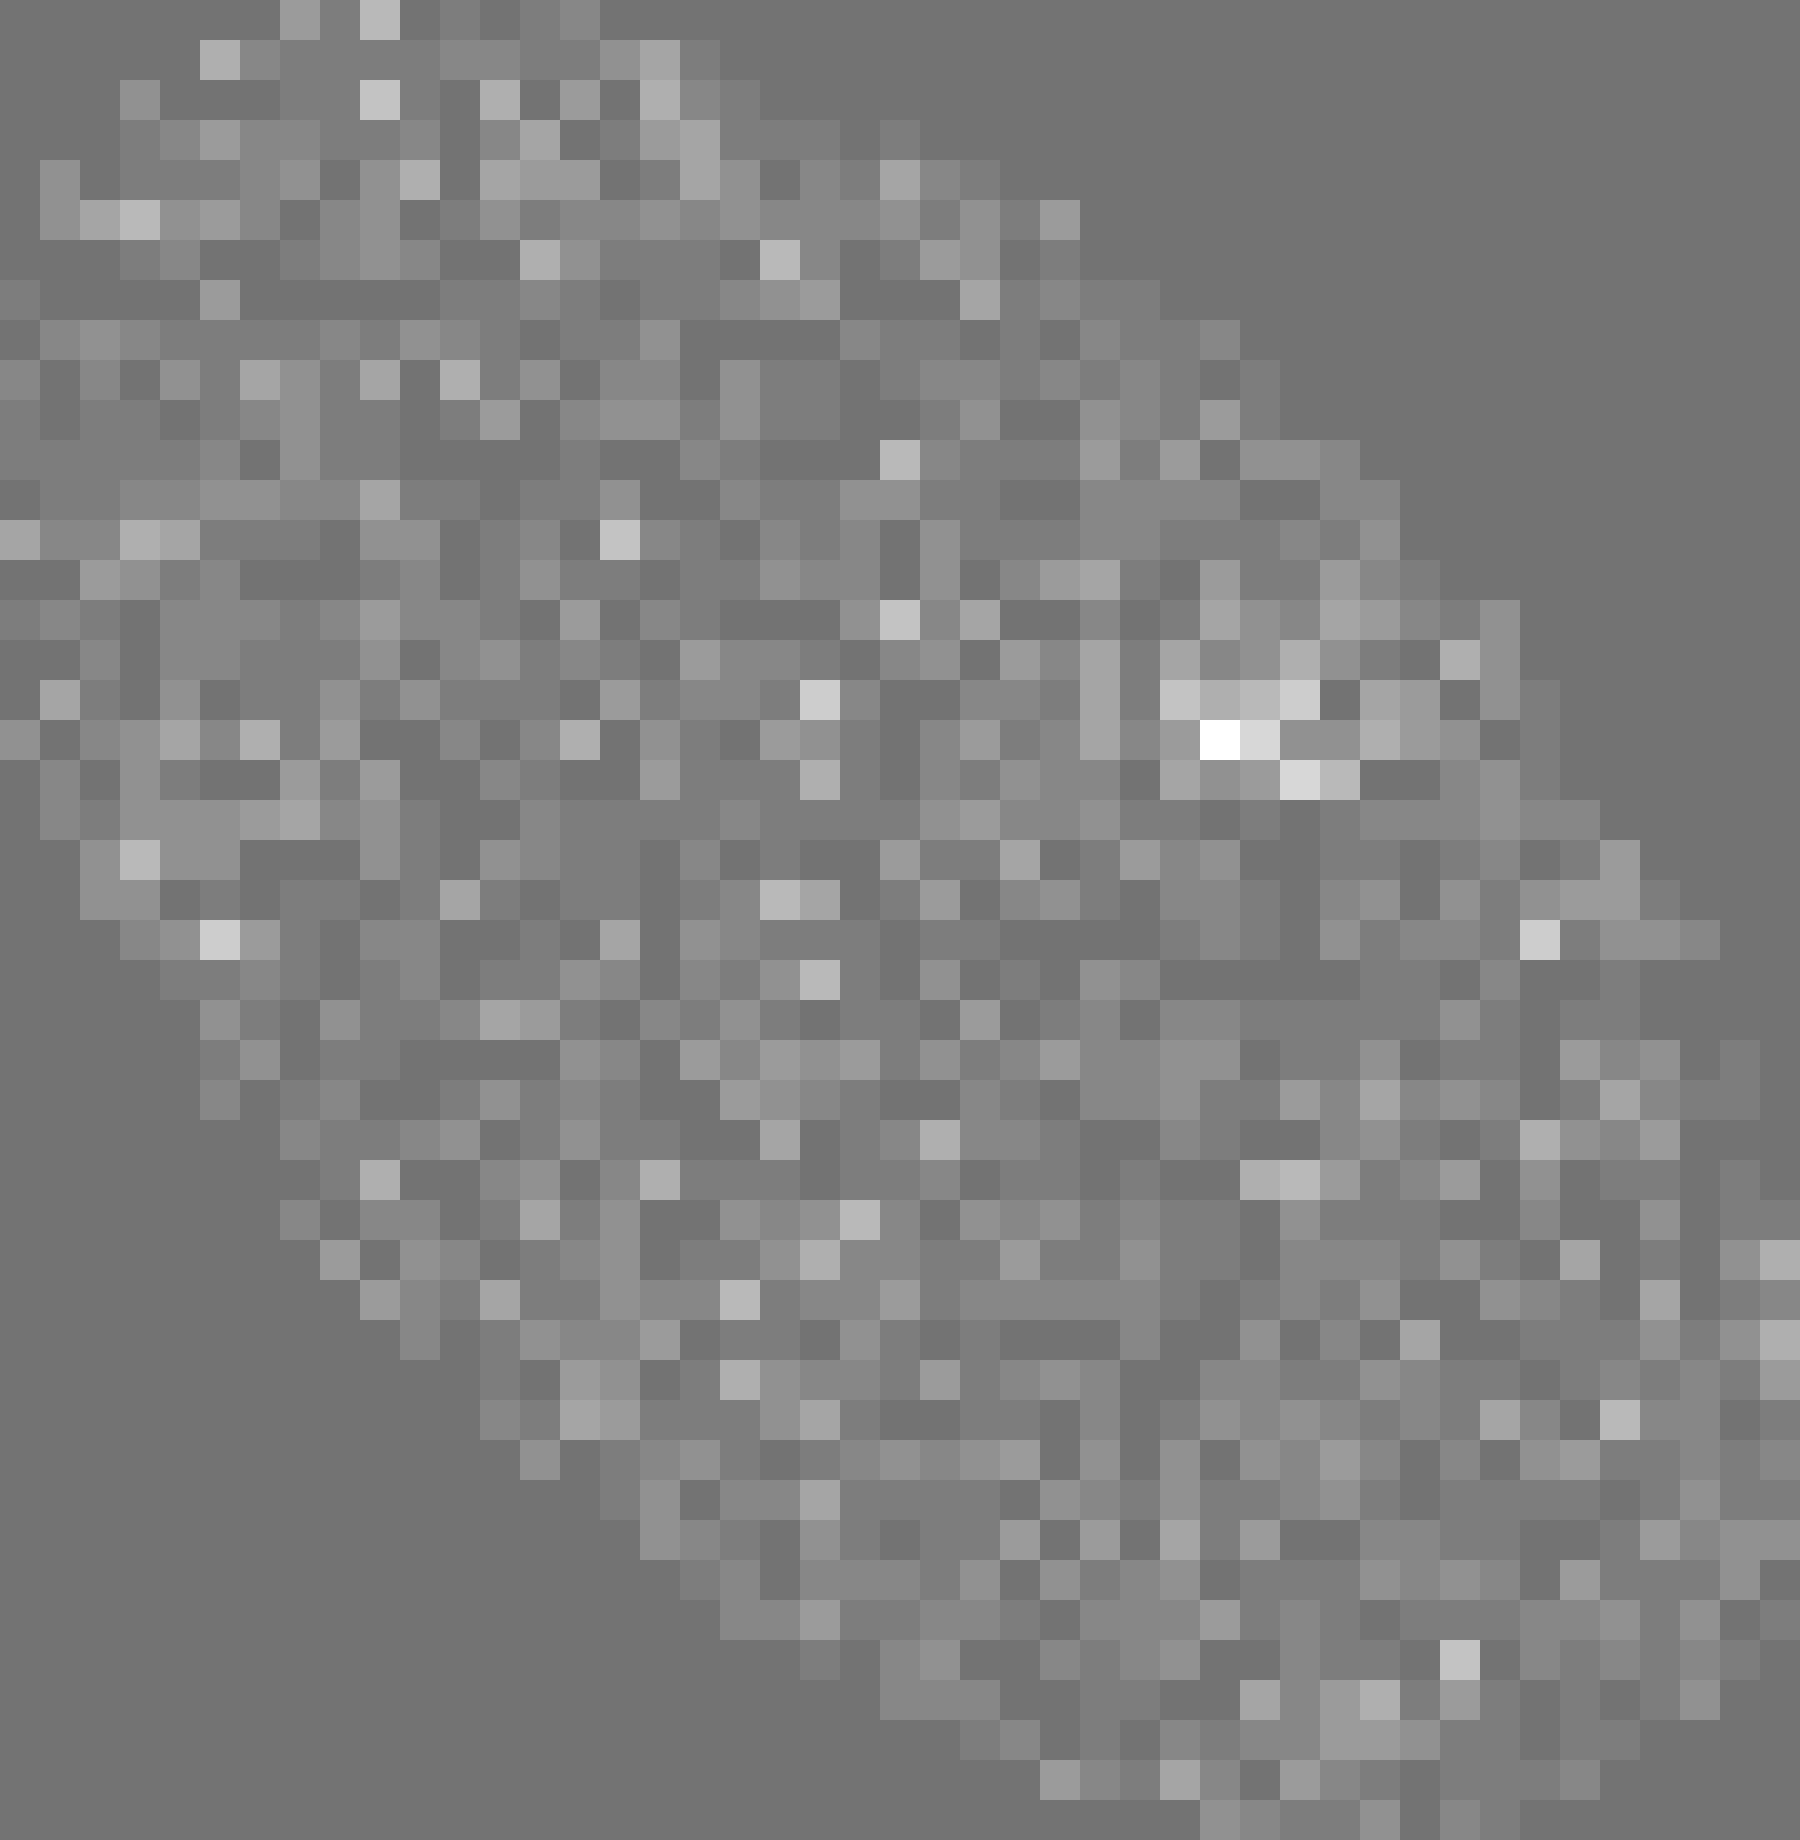
\includegraphics[width=6cm]{Plots/Preprocessed_Image.png}
    \caption{Skewed input image mapped to quadratic pixels}
    \label{fig:preprocessed_image}
\end{figure}



\section{Convolutional Neural Networks}
In the recent years Deep Learning evolved at an incredible rate and generated impressive progress in image classification tasks.
Utilizing the progress this thesis tests the benefit of Convolutional Neural Networks (CNN) for classifying the skewed camera images
by their triggering cosmic particle.
To separate images caused by gammas or hadrons there are many possible architectures for the CNN.
Every architecture is composed of layers with different tasks.
The image will then be passed and transformed from layer to layer till it reaches the last one.

Convolution layers (depicted in the plots as 'c') act as feature generators.
Patterns in the image will be translation invariant recognized.
Pooling layers reduce the feature space by selecting the most important ones.
They are following a convolution layer and will not be depicted in the plots.
Fully connected layers (depicted as 'f') complete the network in the final stages.
They combine the computed features and classify the image at the same time.

To minimize overfitting and maximize generalization different approaches can be used.
For evenly distributed pixel values batch normalization is used.
At the cost of longer training times Dropout layers ('d') can be inserted after any layer.
This will destroy some of the information flowing through the network
and force it to learn distributed representations of every feature making it more robust.
To enable long networks and faster training pretraining will be implemented.
After training small networks for a short time a new untrained layer will be attached.
This process will be iterated until the networks growth reached its final length.
While most of the layers only have to adapt slightly
the new layers can adjust their behaviour according the pretrained network quickly.

\begin{figure}
    \centering
    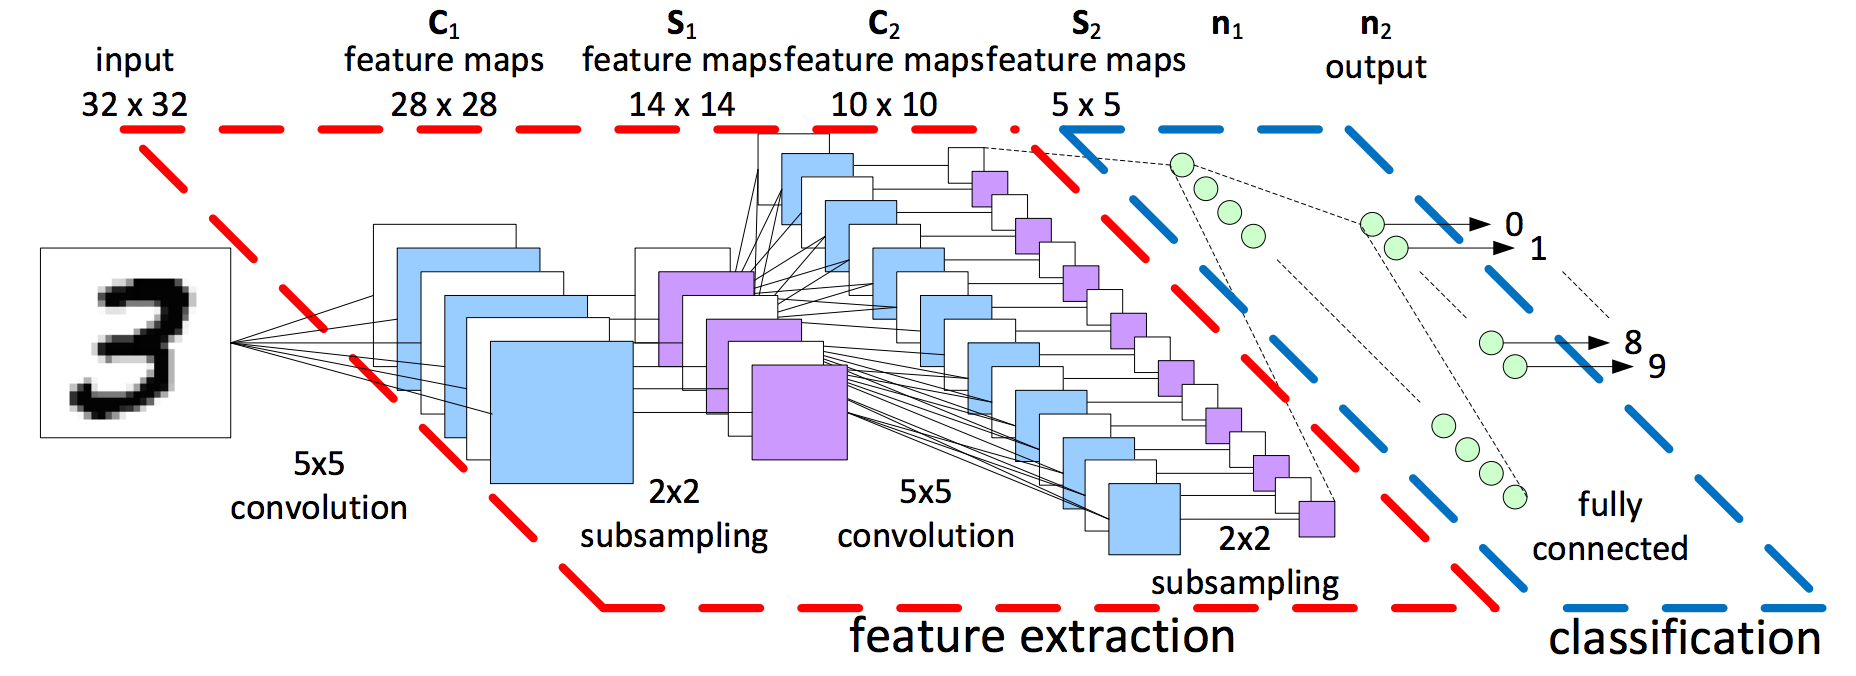
\includegraphics[width=12cm]{Plots/cnn_example.png}
    \caption{Example architecture of a CNN with Convolution, Pooling and Fully connected layers}
    \label{fig:cnn_example}
\end{figure}

\chapter{Optimizing the CNN}%\label{make}

\section{Processing the Images}
For the following steps, a simulated dataset containing roughly \num{800000} gamma events
and \num{400000} hadron events has been used.
Each recorded event holds the counts of every arrived photon for all \num{1440} pixels
for \num{100} consecutive time frames of \num{0.5}\,\si{\nano\second}.
To reduce these \num{144000} variables,
the counts of photons for each pixel have been summed along the time axis (time series summation).

\begin{figure}
    \centering
    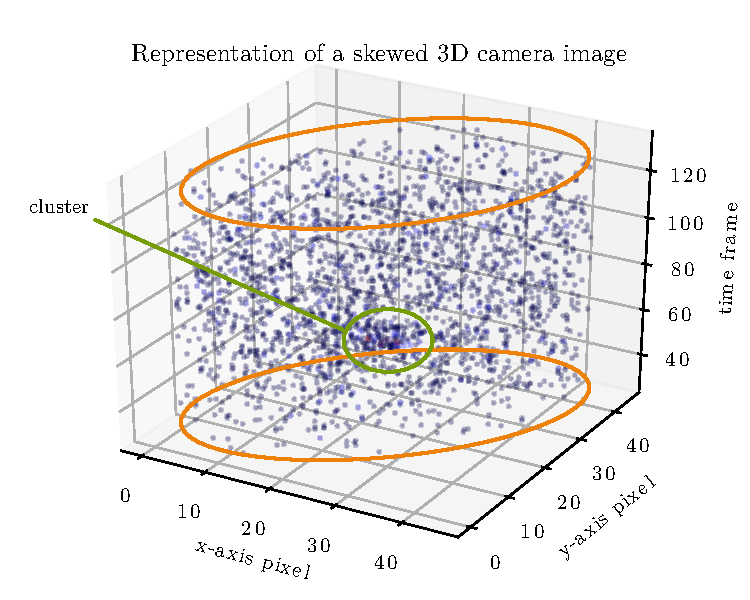
\includegraphics[scale=0.75]{Plots/3d_Camera_Image.pdf}
    \caption{An event contains \num{100} consecutive images of the Cherenkov flash. To minimize the number of variables, all values for a single pixel have been summed up for each event.}
    \label{fig:example_event}
\end{figure}

Naturally, many background photons are contained in the image.
Since the telescope triggers all events in approximately the same time frame,
the photons of the air shower can be cut out by removing preceding and succeeding time frames filled with noise.
This results in cleaner, denoised images for the pattern detection in the CNN.

\begin{figure}
    \centering
    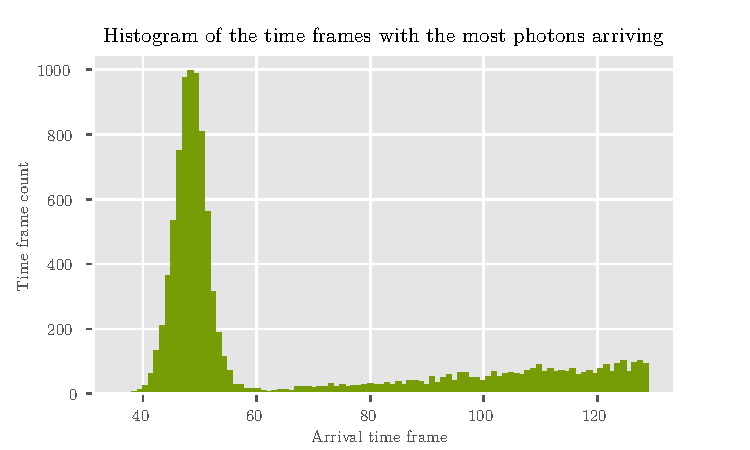
\includegraphics[scale=1]{Plots/Arrivaltimes.pdf}
    \caption{The brightest time frames for \num{10000} events are shown in the histogram. The distribution peaks around the triggering time. By cutting out this cluster, noise can be reduced.}
    \label{fig:arrivaltimes}
\end{figure}

For \num{10000} events, the time frame with the most photons arriving was computed.
These bright time frames most likely contain the events to examine.
Creating a histogram of these time frames,
highlights that the telescope triggers the events between frames \num{35} and \num{60} nearly every time.
As a result, only this range of frames will be used for the denoised images,
dropping all other frames, which contain mostly noise.

In the following paragraph, all architectures will be evaluated on the images
containing all photons as well as the denoised ones.


\section{Comparing Architectures}
In this section each tested network architecture is composed of a convolution layer followed by a pooling layer (c)
and fully-connected layers (f).
The architecture notation follows this example:

\begin{itemize}
\item A \enquote{\texttt{3c\_2f}} architecture translates to a network
starting with three convolution-and-pooling layers and ending with two fully connected layers.
\end{itemize}

There are four important hyperparameters for networks of this kind:

\begin{itemize}
\item The number of images in one batch fed to the network (batch-size)
\item The size of the patch/kernel in the convolution layers (patch-size)
\item The number of feature maps the convolution layers compute (depth)
\item The number of neurons contained in the fully-connected layers (neurons)
\end{itemize}

For all parameters a random grid search was performed over the course of the following steps.
To reduce the impact of random fluctuations in the network's performance caused inter alia by the grid search,
\num{50} networks have been trained for each architecture.

The common procedure of using a separate training, validation and testing dataset has been adopted.
To measure the network's performance, the area under the Receiver-Operating Characteristic (ROC-AUC) \cite{roc_auc} is used.
The training of a network is terminated when the ROC-AUC-score of the validation dataset does not rise anymore (early stopping).

\begin{figure}
\centering
\begin{subfigure}{.5\textwidth}
  \centering
  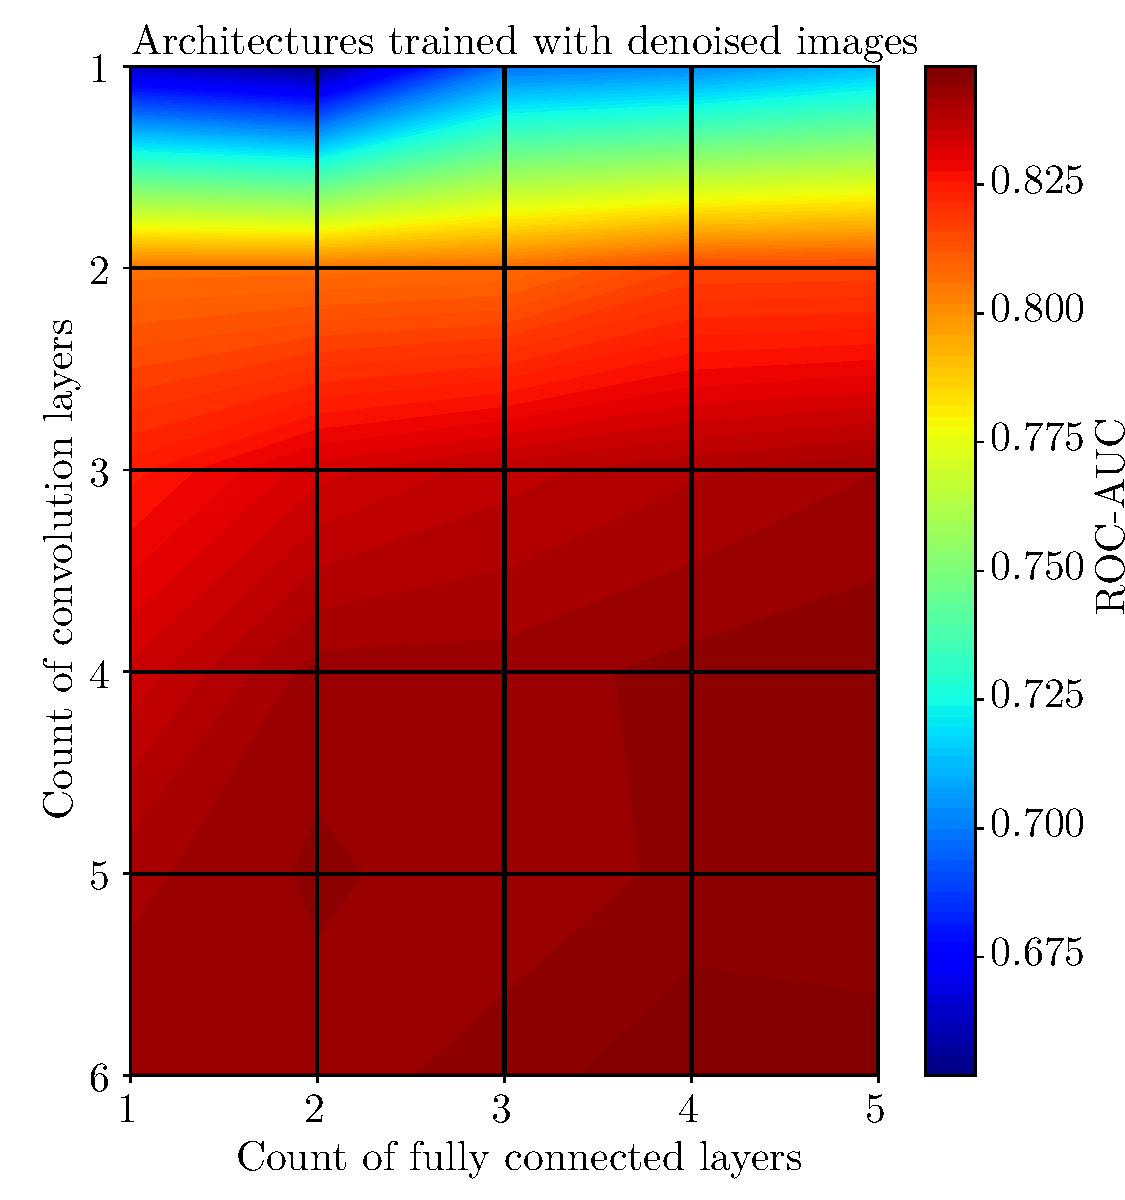
\includegraphics[scale=0.35]{Plots/Architectures_AUC_denoised.pdf}
  \caption{CNNs on denoised images}
  \label{fig:heatmap_denoised}
\end{subfigure}%
\begin{subfigure}{.5\textwidth}
  \centering
  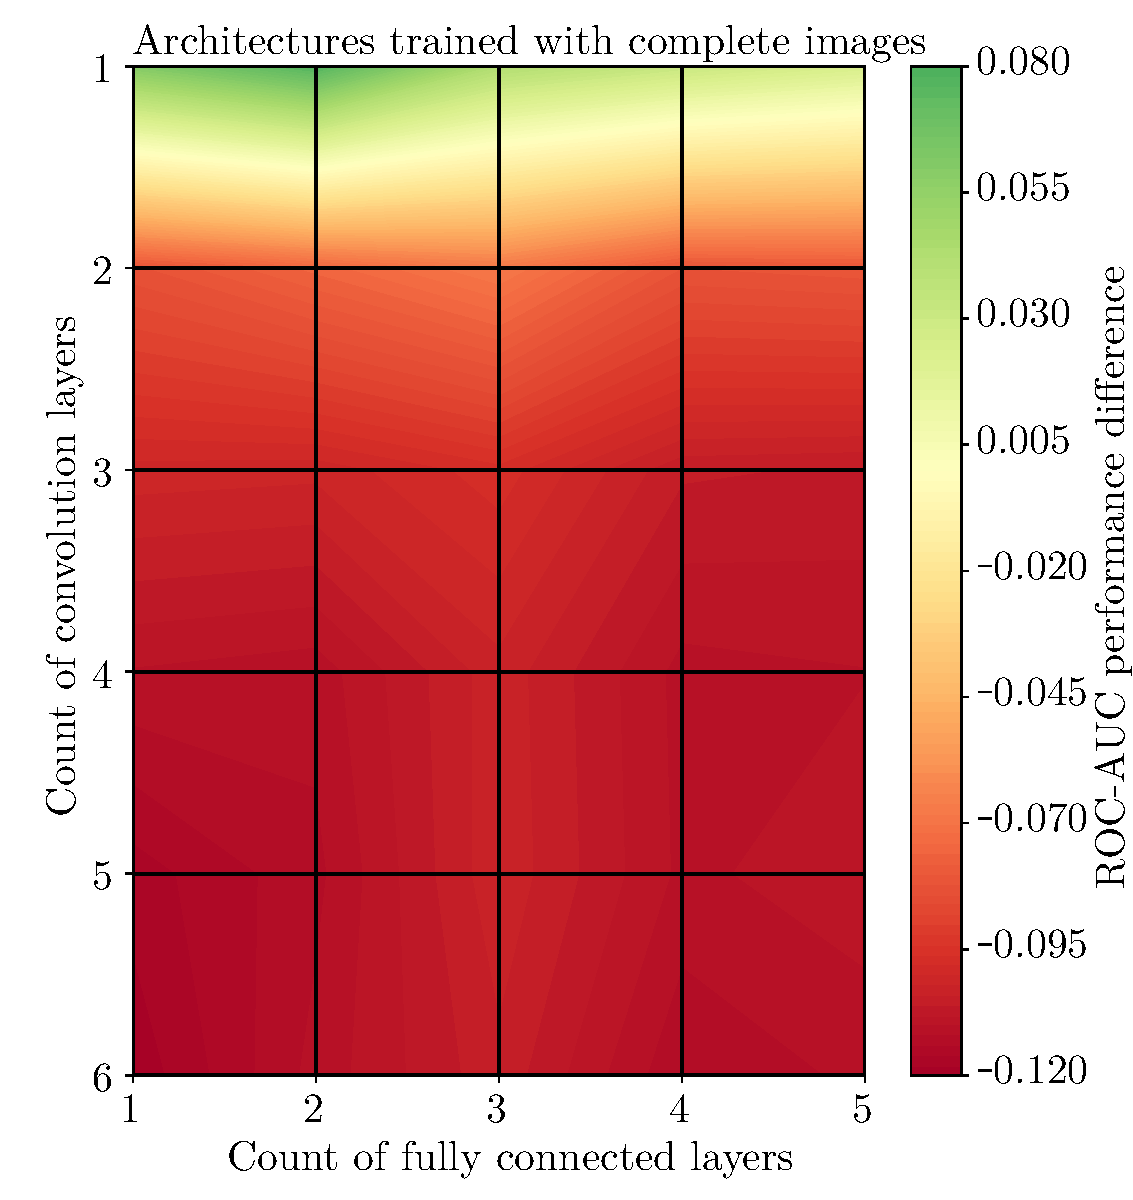
\includegraphics[scale=0.35]{Plots/Architectures_AUC_noised.pdf}
  \caption{CNNs on noisy images}
  \label{fig:heatmap_noised}
\end{subfigure}
\caption{The ROC-AUC performances of \num{30} architectures are compared on both denoised and noisy images. Since denoised images perform better, the second plot shows the difference between the denoised and noisy images' ROC-AUC scores.}
\label{fig:heatmaps}
\end{figure}

By comparing the networks trained on noisy and denoised images, it becomes apparent
that denoised images produce a much more reliable and therefore better network.

Looking at the architectures, it appears unambiguous that deeper networks perform much better than shallow ones.
The number of feature-generating convolution layers seems to have a greater impact
than the number of fully connected layers on the ROC-AUC score.

By examining the best-performing denoised deep network architectures,
only sleight differences can be seen.
Since a sample of only \num{50} trained networks guarantees no statistical certainty,
no distinct best architecture can be proclaimed.

\begin{figure}
    \centering
    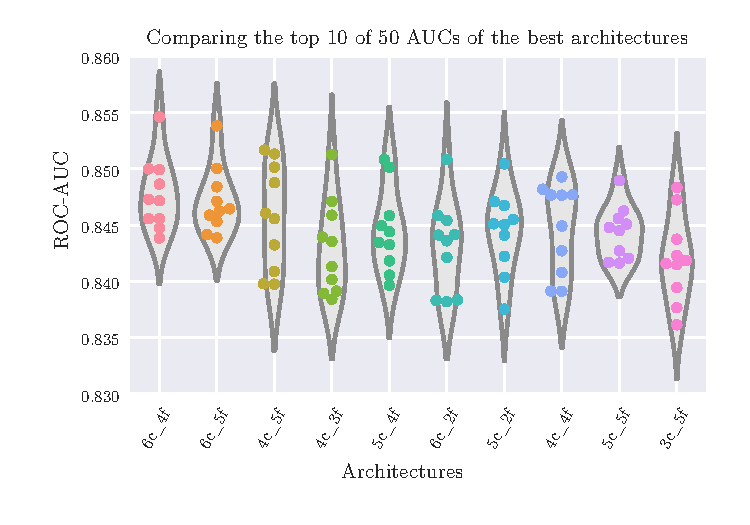
\includegraphics[scale=1]{Plots/Best_denoised_architectures.pdf}
    \caption{For the comparison of the best denoised architectures the \num{10} best performing networks from \num{50} are being compared in this plot.}
    \label{fig:top_cnn_architectures}
\end{figure}

It can be seen that deeper networks perform better on the given task
and the more convolution layers included in the architecture, the higher the ROC-AUC score.
Additionally, using only the important part of the recorded events
and dropping some noise, increases the network's performance as well.

For a meaningful conclusion concerning the architectures, the hyperparameters of the networks will be investigated.
Since the optimal values for the hyperparameters could not be determined beforehand,
all parameters for the above investigations were randomly chosen from a suitable value range.
Therefore a conclusion can be drawn afterwards to narrow this range down or investigate a more promising value range.

Since only the best networks are of interest, the hyperparameters of the high performing ones are investigated.
For this analysis, the performance of all computed networks are compared regardless of their architecture.
As all parameters (batch-size, patch-size, depth and neurons) show only a small impact on the ROC-AUC score,
only small gains in performance can be achieved through optimizing the hyperparameters.
For this reason the random grid search will be performed for further investigations.

\begin{figure}
\centering
\begin{subfigure}{.5\textwidth}
  \centering
  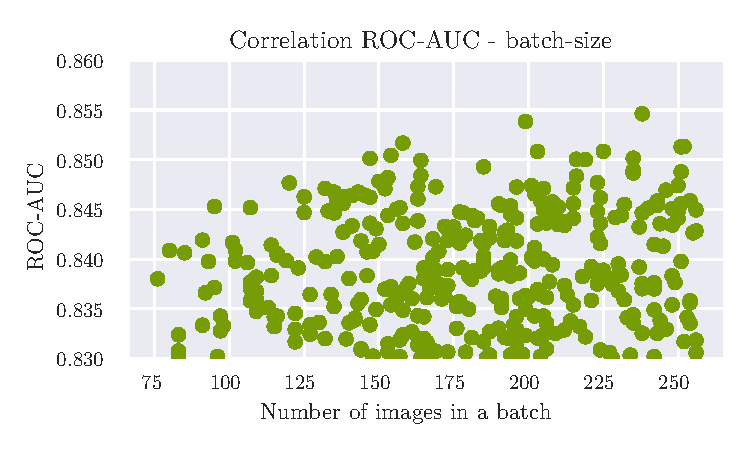
\includegraphics[scale=0.55]{Plots/Best_Hyperparameter_Batch_Size.pdf}
  \caption{Parameter batch-size}
  \label{fig:batch_size}
\end{subfigure}%
\begin{subfigure}{.5\textwidth}
  \centering
  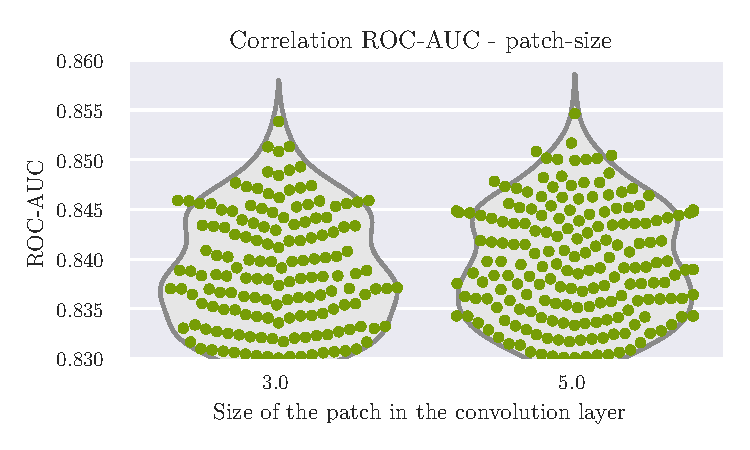
\includegraphics[scale=0.55]{Plots/Best_Hyperparameter_Patch_Size.pdf}
  \caption{Parameter patch-size}
  \label{fig:patch_size}
\end{subfigure}

\centering
\begin{subfigure}{.5\textwidth}
  \centering
  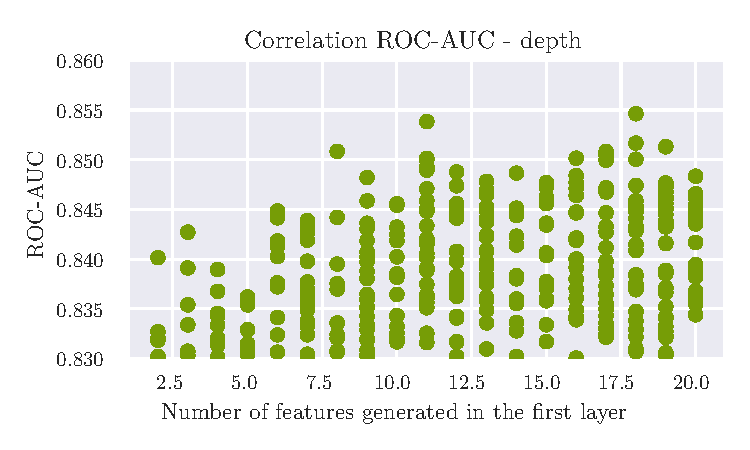
\includegraphics[scale=0.55]{Plots/Best_Hyperparameter_Depth_1.pdf}
  \caption{Parameter depth (first c-layer)}
  \label{fig:depth}
\end{subfigure}%
\begin{subfigure}{.5\textwidth}
  \centering
  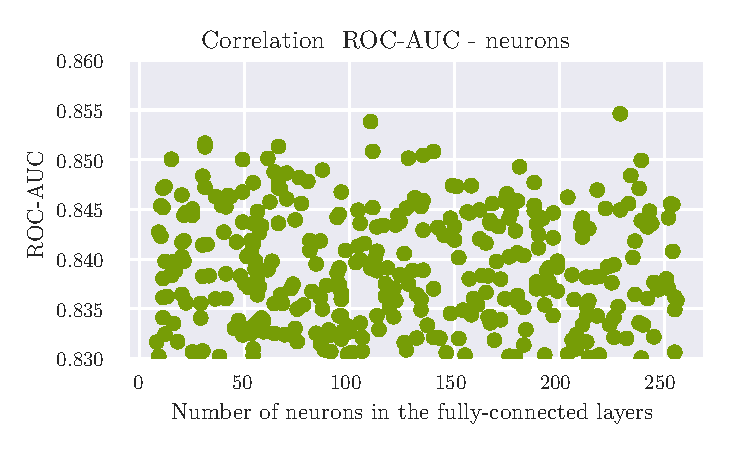
\includegraphics[scale=0.55]{Plots/Best_Hyperparameter_Hidden_Nodes.pdf}
  \caption{Parameter hidden-nodes}
  \label{fig:hidden_nodes}
\end{subfigure}
\caption{Only a small impact on the ROC-AUC can be detected by comparing the hyperparameters. Since optimizing the parameters specifically appears complicated, the random grid search will be utilized henceforth.}
\label{fig:parameter}
\end{figure}



\section{Regularizing the Network}
The best-performing \enquote{\texttt{6c\_4f}} architecture is fixed for further investigations
so that the feature space to explore is reduced.
To stabilize behavior of the network, regularizing dropout layers will be integrated into the network's architecture.

Since the layer can be combined with every existing layer in the network
and can likewise adopt different values for the amount of data to drop out in every layer,
a large feature space has to be evaluated.
As adding dropout to a network extends the training time many times over,
only one dropout layer at once can be tested at every position.
In the first round of testing, a dropout rate of \num{50}\,\% will be used.
Investigating every possible permutation of multiple dropout layers is not possible
because of the size of the feature space that must be explored.

\begin{figure}
    \centering
    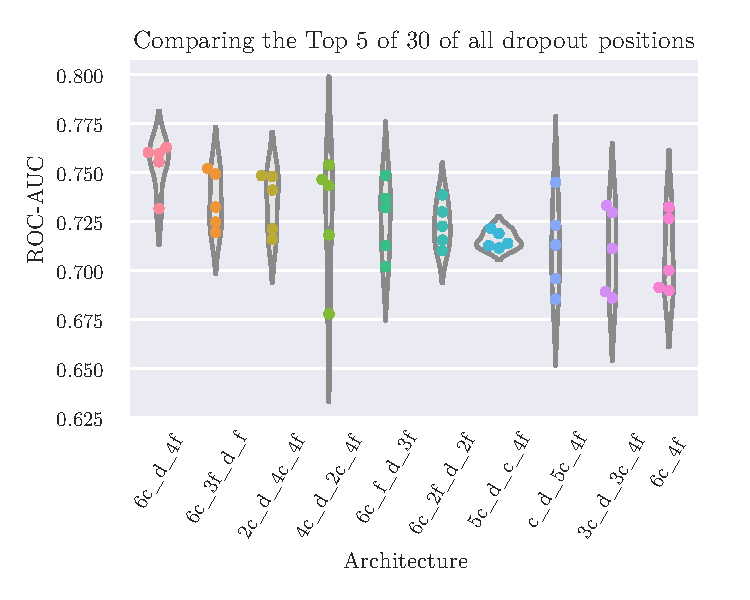
\includegraphics[scale=1]{Plots/Dropout_Positions.pdf}
    \caption{Using dropout layers increases the performance every time, but inserting the layer between the convolution and the fully connected layers, unlocks its potential the most.}
    \label{fig:random_dropout}
\end{figure}

Positioning the dropout layer between the convolution layers and the following fully-connected layers
appears to have the most positive impact on the network's performance.
Regularizing the fully connected layers seems to strengthen the network as well.
On the contrary, dropping too much information in the convolution layers weakens the network overall.
Therefore, the dropout rate is most important, when it is combined with the layer's position.

It has been decided that dropout layers shall be implemented after every layer, but using different dropout rates.
The rates in table \ref{tab:dropout_rates} were taken from corresponding literature \cite{deeplearning}.

\begin{table}
    \centering
    \caption{The chosen dropout rates for the different dropout positions}
    \label{tab:dropout_rates}
    \begin{tabular}{cc}
        \toprule
        {Dropout position}  & {Dropout rate} \\
        \midrule
        c- d -c & 0.90 \\
        c- d -f & 0.75 \\
        f- d -f & 0.50 \\
        \bottomrule
    \end{tabular}
\end{table}

Since dropout prolongs the network's training cycle and increases the difficulty of training deep networks in general,
pretraining is used to enable efficient training of many layers.

A short network containing dropout layers is trained for a few epochs
and the layers adjust their inner values using gradient decent.
Afterwards new layers are appended to the network and the short training epoch starts again.
In this case training epochs consisting of \num{0}, \num{1000}, \num{2000}, \num{5000} and \num{8000} batches are being compared.
To complete the training after the network has grown to its full depth, a normal training epoch with early stopping is used.

\begin{figure}
    \centering
    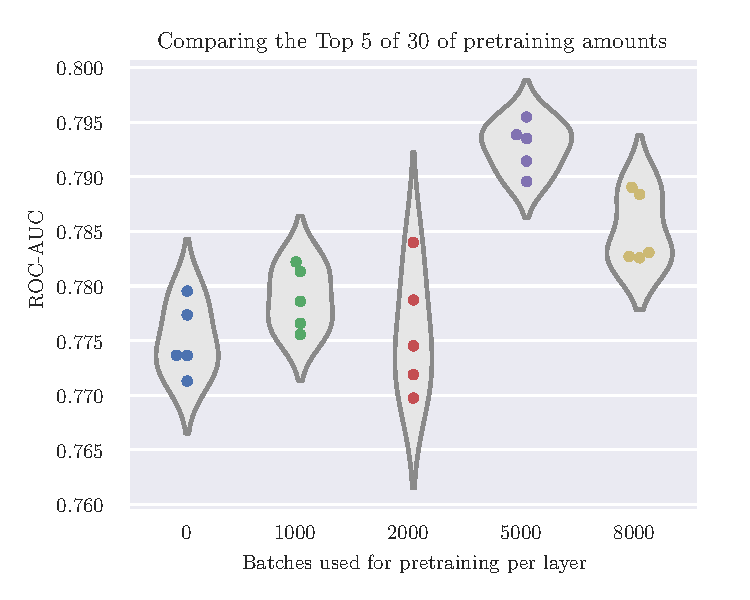
\includegraphics[scale=1]{Plots/Pretraining_Amounts.pdf}
    \caption{Implementing pretraining in the training process increases the network's performance in general. Since too much pretraining appears to be counterproductive, \num{5000}\,batches will be used henceforth.}
    \label{fig:pretraining_amounts}
\end{figure}

Using different amounts of pretraining batches, the results illustrate an increase in the performance
when compared to the networks without pretrained layers.
By pretraining the network too much, there seems to be an decrease in the performance through overfitting.
Therefore, it is advisable to choose the pretraining amount carefully.
In this case \num{5000} batches of images have been chosen.

\chapter{CNNs results}

\section{Comparing the CNN to the current method}

CNN weitestgehend optimiert und nur noch kleinere Fortschritte hier zu erwarten

Deshalb nun Performance des CNN evaluieren

erst ansehen wie sich simulierte Daten verteilen (Histogramm)

Ratio von gamma zu hadron bekannt und verhält sich wie erwartet

viele korrekt simuliert und doch sehr ähnliche events schwer zu unterscheiden

\begin{figure}
    \centering
    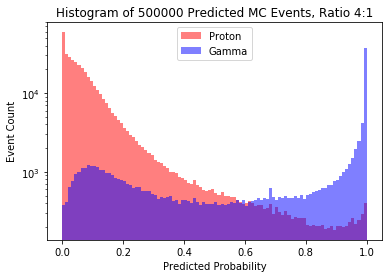
\includegraphics[width=10cm]{Plots/MC_Prediction_Histogram.png}
    \caption{CNN predictions of simulated events}
    \label{fig:histogram_simulated_data}
\end{figure}

histogram vergleich auf echten daten

ähnliche verteilung erwartet nur in der größenordnung unterschiedlich

es stellt sich komplett anderes verhaöten ein

lässt auf missmatch schließen und rückschlüsse auf fehlerhafte ausgangsdaten zulässig

\begin{figure}
    \centering
    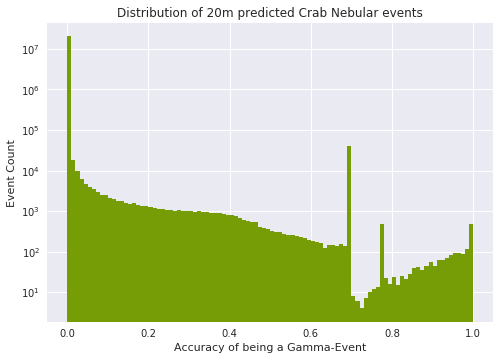
\includegraphics[width=10cm]{Plots/Predicting_real_data.png}
    \caption{CNN predictions of real events}
    \label{fig:histogram_real_data}
\end{figure}

schlussendlich vergleich über theta-plot

erklärung, dass on-off-daten genommen werden und dann die signifikanz der quelle errechnet wird

signifikanz für die messdauer miserabel!

da cnn weitestgehend optimiert, nicht mit optimierung rauszukriegen

\begin{figure}
    \centering
    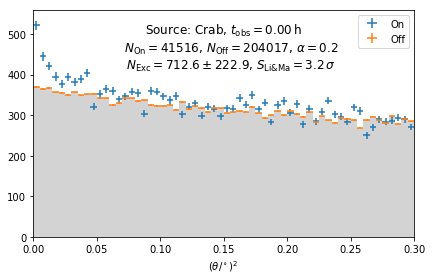
\includegraphics[width=10cm]{Plots/Theta_Plot.png}
    \caption{Theta-Plot for the significance of the crab nebula}
    \label{fig:theta_plot}
\end{figure}


\section{Potential enhancements}

Weitere Verbesserung für das CNN:

Hyperparametersuche unterstützt durch Reinforcementlearning und eigenständiges finden der optimalen Einstellung

3D Convolution über alle nachbarn (hexagonal to 3D)

Einbeziehen der Zeitinformationen (3D Convolution, 4D Convolution, LSTM/RNN)

Verbessern der Monte Carlo Daten:

Missmatches raussieben

Echter Hintergrund verwenden

Klassifizierer verwenden und dann auf vorhergesagten Labels CNN trainieren (kein Missmatch nur Fehlinformationen)


%\appendix
% Hier beginnt der Anhang, nummeriert in lateinischen Buchstaben
%\chapter{Ein Anhangskapitel}

Hier könnte ein Anhang stehen, falls Sie z.B. Code, Konstruktionszeichnungen oder Ähnliches mit in die Arbeit bringen wollen. Im Normalfall stehen jedoch alle Ihre Resultate im Hauptteil der Bachelorarbeit und ein Anhang ist überflüssig.


\backmatter
\printbibliography

\cleardoublepage
\thispagestyle{empty}
\section*{Eidesstattliche Versicherung}
Ich versichere hiermit an Eides statt, dass ich die vorliegende Abschlussarbeit mit dem Titel \enquote{\thetitle} selbstständig und ohne unzulässige fremde Hilfe erbracht habe.
Ich habe keine anderen als die angegebenen Quellen und Hilfsmittel benutzt, sowie wörtliche und sinngemäße Zitate kenntlich gemacht. 
Die Arbeit hat in gleicher oder ähnlicher Form noch keiner Prüfungsbehörde vorgelegen.

\vspace*{1cm}\noindent
\begin{center}
  \begin{tabular}{@{}p{0.4\textwidth}@{\hspace{0.15\textwidth}}p{0.4\textwidth}@{}}
  \rule{\linewidth}{0.25pt}& \rule{\linewidth}{0.25pt}\\
  Ort, Datum & Unterschrift
  \end{tabular}
\end{center}

\subsection*{Belehrung}
Wer vorsätzlich gegen eine die Täuschung über Prüfungsleistungen betreffende Regelung einer Hochschulprüfungsordnung verstößt, handelt ordnungswidrig.
Die Ordnungswidrigkeit kann mit einer Geldbuße von bis zu \SI[round-mode=places, round-precision=2]{50000}{€} geahndet werden. 
Zuständige Verwaltungsbehörde für die Verfolgung und Ahndung von Ordnungswidrigkeiten ist der Kanzler/die Kanzlerin der Technischen Universität Dortmund. 
Im Falle eines mehrfachen oder sonstigen schwerwiegenden Täuschungsversuches kann der Prüfling zudem exmatrikuliert werden \mbox{(\S\,63 Abs. 5 Hochschulgesetz --HG--).}

Die Abgabe einer falschen Versicherung an Eides statt wird mit Freiheitsstrafe bis zu 3 Jahren oder mit Geldstrafe bestraft.

Die Technische Universität Dortmund wird ggf.\ elektronische Vergleichswerkzeuge (wie z.\,B.\ die Software \enquote{turnitin}) zur Überprüfung von Ordnungswidrigkeiten in Prüfungsverfahren nutzen. \\[\baselineskip]

\noindent Die oben stehende Belehrung habe ich zur Kenntnis genommen.\\[1cm]
\begin{center}
\begin{tabular}{@{}p{0.4\textwidth}@{\hspace{0.15\textwidth}}p{0.4\textwidth}@{}}
\rule{\linewidth}{0.25pt}& \rule{\linewidth}{0.25pt}\\
Ort, Datum & Unterschrift
\end{tabular}
\end{center}

\end{document}
